\documentclass[12pt]{article}
\usepackage{graphicx}
\usepackage{gensymb}

\begin{document}
\graphicspath{ {images/} }
\section*{About Network Visualization}

In the third tab \textit{Network Visualization} you can have a deep view of the model and test result.

\subsection{Show architecture}
After loading a network model, you can click the button \textit{show architecture}, you will see an image showing the architecture of the network. 

\subsection{Show layer weights}
After load both a network model and test datasets, the layers will be automatically shown in the list on the left side. You can check on either the filter radio button to show weights of layers, or check on the maps radio button to show feature maps. Then you select the desired layer, if this layers has activation, there will be a plot of the weights or feature maps on the right side. You can also slide the horizontal slider bar at the bottom to change the number of slices to show on.
\begin{figure}[htbp]	
	\centering
	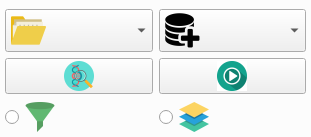
\includegraphics{visualization_in.png}
	\caption[Network Visualization Input]{Network Visualization Input}
	\label{fig:visualization_in}
\end{figure}

\subsection{Show subsection}
If the network has two input layers, it is supported in the GUI to show subsection individually. You need to check on plot either the first or the second input. There are two parameters $\alpha$ and $\gamma$ used for adjusting showing subsection. $\alpha$ is for \textit{l2}-regularization on the wanted input image to obtain feasible results; $\gamma$ is for step size for the proximal gradient algorithm  And start \textit{show subsection}.

\subsection{Show prediction result}
After perform prediction, if the network is used for segmentation, you can take a look at the segmentation masks and artifacts. Or if the network is used only for classification, you can also have a look at the confusion matrix as well. The trigger item is in the drop down box \textit{Showing Test Result}.
\begin{figure}[htbp]	
	\centering
	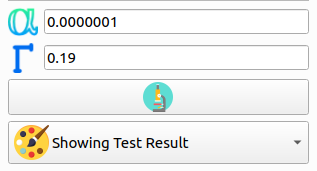
\includegraphics{visualization_out.png}
	\caption[Network Result Visualization]{Network Result Visualization}
	\label{fig:visualization_out}
\end{figure}

\end{document}
